\documentclass[a4paper, 10pt]{article}

%\usepackage{scalefnt}
%\usepackage{parcolumns}

\usepackage{newclude}
% Zum Einbinden in die Zusammenfassungs-files

\usepackage{amsmath,amsthm,amsfonts,amssymb} % Verbesserter Mathesatz
\usepackage{algorithm2e}
\usepackage{bigfoot} % komplexe Fußnotenapparate(Fußnoten in Fußnoten und andere Späße)%
\usepackage{colortbl}
\usepackage[T1]{fontenc} % normaler erweitere Zeichnesatz
\usepackage{framed, color}  % Ramenpaket für zum Einfügen von schönen Ramen
\usepackage{graphicx}
\usepackage{hyperref} %used for link to creative commons license
\usepackage{listings} %for code-listings (inkl. Tab-Styling)
\usepackage{marvosym}
\usepackage{marginnote}
\usepackage{microtype} % div. Verbesserungen des Schriftsatzes (Grauwert, opt. Randausgleich, Zeilenumbruch)
%\usepackage{multirow}
\usepackage{multicol} %use this with next line for vertical divided environment
%\setlength\columnseprule{.4pt}:465
\usepackage[ngerman]{babel} % Neue Rechtschreibung
\usepackage{pifont}
\usepackage[sans]{dsfont} %für alternative Mengensymbole
\usepackage{stmaryrd} %u.a. für \lightning
\usepackage{tikz} % für Diagramme(Dia!) und Bilder (z.B. *.eps)/für ER-Diagramme/für UML-Diagramme
%\usepackage{tikz-er2} %  er-diagramme
\usepackage{tikz-uml} % uml-Diagramme
\usepackage{units} % z.B. fuer \nicefrac{}{}
\usepackage[utf8]{inputenc} % utf8 für den Editor
\usepackage{wasysym} %u.a. für \lightning
\usepackage{xcolor}


\usetikzlibrary{shapes,decorations,arrows,fit,backgrounds} %Zum diversen zeichen%
%\usetikzlibrary{automata} % für den CFlipper, wenn es den soweit ist			%
\usetikzlibrary{positioning} % positionierung
%\usetikzlibrary{shadows} % fuer schoene schlagschatten
\usetikzlibrary{automata} % für Automaten

%%%%%%%%%%%%%%%%%%%%%%%%%%%
%  Formatierung der Seite
%%%%%%%%%%%%%%%%%%%%%%%%%%%
\usepackage{fancyhdr}
\pagestyle{fancy}		% für den footer										%
\renewcommand{\headrulewidth}{0pt} % damit oben kein dummer Strich kommt		%
\fancyhead{}
\topmargin -2cm 		% Oberer Rand											%
\textheight 25cm		% Texthöhe												%
\textwidth 16.0 cm		% Textbreite											%
\oddsidemargin -0.1cm 	% Warum?												%
\newcommand{\Gruppe}[2]
{
	\lfoot{#1}
	\rfoot{#2}
}
\colorlet{shadecolor}{gray!25} % Farbe für graue Box definieren
%%%%%%%%%%%%%%%%%%%%%%%%%%%%%%%%%%%%%%%%%%%%%%%%%%%%%%%%%%%%%%%%%%%%%%%%%%%%%%%%%
%Farben die definiert werden zum schreiben und zeichnen							%
%%%%%%%%%%%%%%%%%%%%%%%%%%%%%%%%%%%%%%%%%%%%%%%%%%%%%%%%%%%%%%%%%%%%%%%%%%%%%%%%%
\xdefinecolor{schwarz}{HTML}{000000}
\xdefinecolor{dunkelGruen}{HTML}{007D00}
\xdefinecolor{dunkelBlau}{HTML}{0000A0}
\xdefinecolor{dunkelRot}{HTML}{A00000}
\xdefinecolor{dunkelGelb}{HTML}{FFAA00}
\xdefinecolor{hellesGelb}{HTML}{FFCC00}
\colorlet{dGreen}{dunkelGruen}
\colorlet{dBlue}{dunkelBlau}
\colorlet{dRed}{dunkelRot}
\colorlet{dYellow}{dunkelGelb}

%%%%%%%%%%%%%%%%%%%%%%%%%%%%%%%%%%%%%%%%%%%%%%%%%%
%Farbliche Ausgaben:
%Parameter #1: Text oder Mathematische formel...
%z.B. : \gruen{Hallo Welt Test!}
%%%%%%%%%%%%%%%%%%%%%%%%%%%%%%%%%%%%%%%%%%%%%%%%%%

\newcommand{\yellow}[1]{\textcolor{dYellow}{#1}}
\newcommand{\gray}[1]{\textcolor{gray}{#1}}
\newcommand{\red}[1]{\textcolor{red}{#1}}
\newcommand{\green}[1]{\textcolor{green}{#1}}
\newcommand{\blue}[1]{\textcolor{blue}{#1}}
\newcommand{\dGreen}[1]{\textcolor{dGreen}{#1}}
\newcommand{\dBlue}[1]{\textcolor{dBlue}{#1}}
\newcommand{\dRed}[1]{\textcolor{dRed}{#1}}

%%%%%%%%%%%%%%%%%%%%%%%%%%%%%%%%%%%%%%%%%%%%%%%%
%Konfiguration für das darstellen von Quelltext
%%%%%%%%%%%%%%%%%%%%%%%%%%%%%%%%%%%%%%%%%%%%%%%%
\lstset
{
	language=Java, % oder C++, Pascal, {[77]Fortran}, ...
	numbers=left, % Position der Zeilennummerierung
	firstnumber=auto, % Erste Zeilennummer
	basicstyle=\ttfamily, % Textgröße des Standardtexts
	keywordstyle=\ttfamily\color{dRot}, % Formattierung Schlüsselwörter
	commentstyle=\ttfamily\color{dGruen}, % Formattierung Kommentar
	stringstyle=\ttfamily\color{dBlau}, % Formattierung Strings
	numberstyle=\tiny, % Textgröße der Zeilennummern
	stepnumber=1, % Angezeigte Zeilennummern
	numbersep=5pt, % Abstand zw. Zeilennummern und Code
	aboveskip=15pt, % Abstand oberhalb des Codes
	belowskip=11pt, % Abstand unterhalb des Codes
	captionpos=b, % Position der Überschrift
	xleftmargin=10pt, % Linke Einrückung
	frame=single, % Rahmentyp
	breaklines=true, % Umbruch langer Zeilen
	showstringspaces=false, % Spezielles Zeichen für Leerzeichen
	tabsize=2,
	texcl=true
}

%%%%%%%%
% Kopf
%%%%%%%%
\newcommand{\Header}[3]
{
	{\footnotesize \parindent0em
		{\sc Universität Konstanz}                \hfill #1 \\
		{\sc Fachbereich Informatik \& Informationswissenschaft} \hfill #2 \\
		#3 \hfill \today
	}
}

%%%%%%%%%%%%%%%%%%%%%%%
% load some java code
% \loadJava{file}
%%%%%%%%%%%%%%%%%%%%%%%
\newcommand{\loadJava}[1]
{
	\lstinputlisting[language=Java]{#1.java}
}

%%%%%%%%%%%%%%%%%%%%%%%
% load some cpp code
% \loadCpp{file.cpp}
%%%%%%%%%%%%%%%%%%%%%%%
\newcommand{\loadCpp}[1]
{
	\lstinputlisting[language=C++]{#1}
}

%%%%%%%%%%%%%%%%%%%%%%%%%%%%%
% load some code
% \loadCode{Python}{file.py}
%%%%%%%%%%%%%%%%%%%%%%%%%%%%%
\newcommand{\loadCode}[2]
{
	\lstinputlisting[language=#1]{#2}
}

%%%%%%%%%%%%%%%%%%%%%%%%%%%%%%%%%%%%%%%%%%%%%%%%%%%%%%%%%%%%%%%%%%%%%%%
% some symbols
%%%%%%%%%%%%%%%%%%%%%%%%%%%%%%%%%%%%%%%%%%%%%%%%%%%%%%%%%%%%%%%%%%%%%%%
\newcommand{\correct}{\green{\text{\ding{52}}}} %for use in text and math
\newcommand{\wrong}{\red{\text{\ding{56}}}} %for use in text
\newcommand{\tflash}{$\yellow{\lightning}$} %for use in text
\newcommand{\mflash}{\yellow{\lightning}} %for use in math
\newcommand{\follows}{$\Rightarrow$} %used so often...
\newcommand{\good}{\item[\dGreen{\ding{58}}]} %an item with a green plus as bullet point
\newcommand{\bad}{\item[\red{\Emailct}]} %better icon for bad items
\newcommand{\note}[1]{\red{\marginnote{#1}}} %add a red margin note
\newcommand{\fitem}{\item[\follows]} %items with a follows arrow
\newcommand{\hm}{\ensuremath{\overset{-\mkern-11mu-\mkern-3.5mu\rhook}{\smash{\odot}\rule{0ex}{.46ex}}\underline{\hspace{0.5em}}\overset{-\mkern-11mu-\mkern-3.5mu\rhook}{\smash{\odot}\rule{0ex}{.46ex}}}}

%%%%%% make emph bold instead of italic %%%%%
\makeatletter
\DeclareRobustCommand{\em}{%
  \@nomath\em \if b\expandafter\@car\f@series\@nil
  \normalfont \else \bfseries \fi}
\makeatother

%%%%%%%%%%%%%%%%%%%%%%%%%%%%%%%%%%%%%%
% languages for \loadCode
%ABAP		IDL				Plasm
%ACSL		inform			POV
%Ada		Java			Prolog
%Algol		JVMIS			Promela
%Ant		ksh				Python
%Assembler	Lisp			R
%Awk		Logo			Reduce
%bash		make			Rexx
%Basic		Mathematica1	RSL
%C			Matlab			Ruby
%C++		Mercury			S
%Caml		MetaPost		SAS
%Clean		Miranda			Scilab
%Cobol		Mizar			sh
%Comal		ML				SHELXL
%csh		Modula-2		Simula
%Delphi		MuPAD			SQL
%Eiffel		NASTRAN			tcl
%Elan		Oberon-2		TeX
%erlang		OCL				VBScript
%Euphoria	Octave			Verilog
%Fortran	Oz				VHDL
%GCL		Pascal			VRML
%Gnuplot	Perl			XML
%Haskell	PHP				XSLT
%HTML		PL/I
%%%%%%%%%%%%%%%%%%%%%%%%%%%%%%%%%%%%%%

\begin{document}

\Gruppe{Stephan Heidinger}{fses 07}
\Header{Functional Safety in Embedded Systems}{Session 07 - Fault and Hazard Analysis Techniques}{Stephan Heidinger}

%\begin{shaded}
%Dieses Dokument wurde unter der Creative Commons - Namensnennung-NichtKommerziell-Weitergabe unter gleichen Bedingungen (\textbf{CC by-nc-sa}) veröffentlicht. Die Bedingungen finden sich unter \href{http://creativecommons.org/licenses/by-nc-sa/3.0/de}{diesem Link}. \\
%\centerline{
\includegraphics[scale=1]{../cc-by-nc-sa.png} }
%\end{shaded}

%\textit{\ensuremath{\overset{-\mkern-11mu-\mkern-3.5mu\rhook}{\smash{\odot}\rule{0ex}{.46ex}}\underline{\hspace{0.5em}}\overset{-\mkern-11mu-\mkern-3.5mu\rhook}{\smash{\odot}\rule{0ex}{.46ex}}}
%Find any errors? Please send them back, I want to keep them!}

%\section*{something}

%\section*{more}

\section*{Techniques for Safety Assessment}
\subsection*{Introduction}
\begin{description}
    \item[hazard:] condition that has potentially harmful consequences (for people or environment)
    \item[accident:] hazard, that results in harmful consequences
    \item[accidental event:] event, that leads up to an accident
    \item[incident, near accident, near miss:] an event, that could be an accident, but nothing bad happened
    \item[severity:] impact of possible hazard
    \item[risk:] severity and possibility
\end{description}

\subsection*{Hazard Analysis}
\begin{itemize}
    \item collection of different techniques
    \begin{description}
        \item[inductive] start by considering the initiating causes of given hazard, trace them forward through event propagation to corresponding safety consequences \follows Failure Mode Effects Analysis
        \item[deductive] consider unintended behavior of system, trace it backward to corresponding causes \follows Fault Tree Analysis (FTA)
    \end{description}
\end{itemize}

\subsubsection*{Fault Tree Analysis (FTA)}
\begin{itemize}
    \item used in all fields of safety engineering
    \item deductive analytical technique
    \item \emph{top-level event} (TLE) is specified and the system is analyzed for possible chain of \emph{basic events}, that may cause the TLE
    \item analyze cause of hazard, not find hazards
    \item typical representation is a \emph{fault tree} (FT), makes use of logical gates (AND, OR)
    \begin{center}
    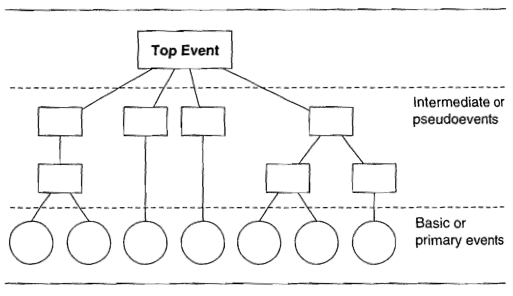
\includegraphics[width=.49\textwidth]{images/FTsimple.png}
    \end{center}
    \newpage
    \begin{multicols}{2}
    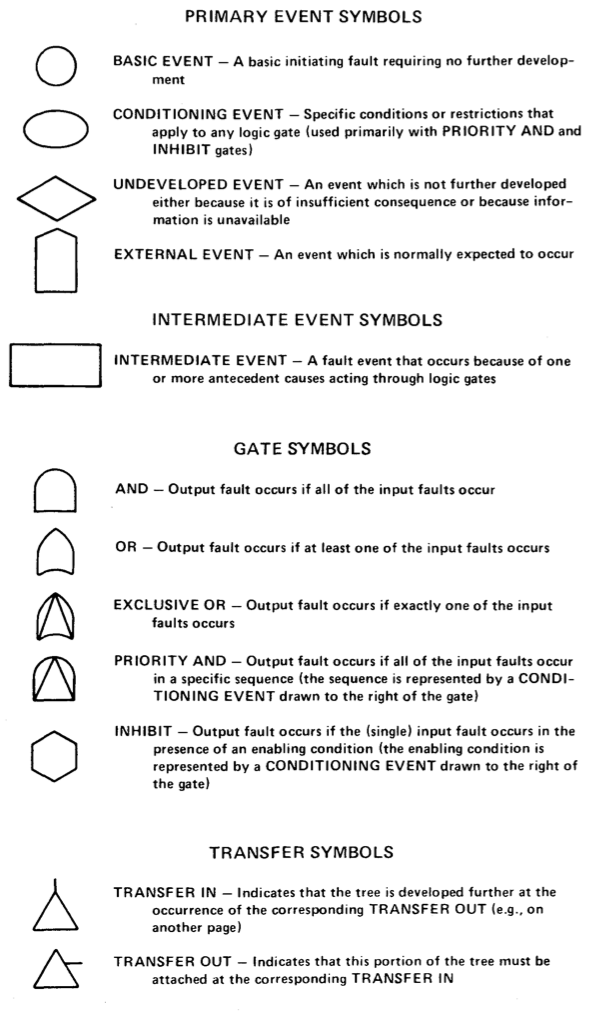
\includegraphics[width=.49\textwidth]{images/FTsymbols.png}
    \columnbreak
    \begin{description}
        \item[AND] both events are required to occur
        \item[OR] alternate causes
        \item[inhibit, NOT] less common
        \item[basic events] leafs (depicted by a circle)
        \item[intermediate events] nodes between leafs and root (depicted by a square)
        \item[undeveloped event] not further analyzed, because not important (depicted by a diamond)
        \item an event needs to be developed considering \emph{immediate}, \emph{necessary} and \emph{sufficient} results
        \item[elementary faults] \follows basic events
        \item[transfer symbols] may link different parts of tree
        \item[inhibit gates, conditioning events] can be used to constrain the ways that faults are propagated inside FT
        \item[dynamic gates] like \emph{priority AND} \follows temporal constraints
    \end{description}
    \end{multicols}
    \item fault tree can be shown as tree, formula or truth table\\ tree is most readable
    \item important notations:
    \begin{description}
        \item[scope \& boundary] define, which parts of the system will be included in the analysis \& under which hypothesis/ operational constraints the system will be analyzed
        \begin{description}
            \item[boundary] initial state of system, and assumptions about environment
        \end{description}
        \item[level of resolution] level of detail used to trace back an event (which must be traced farther down, which can be left undeveloped)
    \end{description}
    \item there may be different choices for intermediate events
    \item \emph{localized} fault \follows \emph{primary, secondary, command} faults are investigated
    \begin{description}
        \item[primary] fault is in an environment, the component is specified for
        \item[secondary] fault is in an environment, the component is not specified for
        \item[command] fault is due to correct operation, but at the wrong time
    \end{description}
    \item qualtitative analysis can be conducted after tree has been completed
    \begin{itemize}
        \item \emph{Minimal Cut Set} minimal set of events needed for the top event \follows top event, OR, all events needed
        \item shows up weaknesses of system
    \end{itemize}
    \item quantitative analysis can be conducted after tree has been completed
    \begin{itemize}
        \item use minimal cut set to calculate probability of the top event (from the probability of basic events)
    \end{itemize}
    \begin{center}
    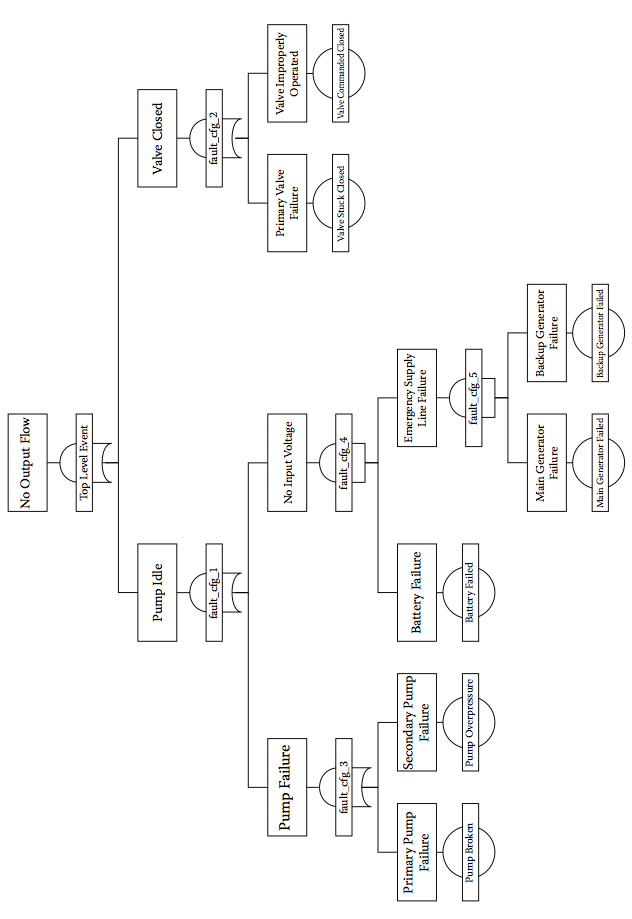
\includegraphics[width=\linewidth]{images/FTex.png}
    \end{center}
    \item automatic FT synthesis possible if design is purely hardware
    \item software FTA
    \begin{itemize}
        \item verification \follows code already has to be written {\tiny (Or the logic has to be fully described)}
        \item if loops present in software \follows human assistance needed
    \end{itemize}
    \item quantitative analysis very costly \follows may be more feasible, if some designs and only small differences
    \item additional analysis needed for effective safety program
    \item suited for discrete events (valve open/ close) but not for rate- or time- dependent events
    \bad not suited for \emph{phased mission} (missions, where there are different phases) (one fault tree needed for each phase, as same components may be used in different configurations and environments)
\end{itemize}

\subsubsection*{Failure Mode and Effect Analysis (FMEA)}
\begin{itemize}
    \item inductive technique
    \item introduced 1940 by US military, later for Apollo (NASA)
    \item extensive spread in variety of domains
    \item starts with identification of failure modes \follows forward reasoning \follows asses their effects on complete system
    \item usually consider effects on same level (and usually one level higher)
    \item also \emph{scope} and \emph{boundary} \follows by safety engineer and take user requirements into account
    \item can be applied to hardware component level or at functional level
    \item typically consider only single faults, combinations can be considered in particular cases
    \item extension: \emph{Failure Modes, Effects and Criticality Analysis} (FMECA)
    \begin{itemize}
        \item also take criticality of consequences of component failures into account
        \item can identify weaknesses in development process (e.g. assembly or manufacturing) \follows \emph{process FMECA}
    \end{itemize}
    \item results \follows FMEA-table
    \item results of FMEA \follows \emph{Failure Mode Effects Summary} (FMES) \follows failure modes leading so same effect are grouped
\end{itemize}

\subsubsection*{HAZard and OPerability studies (HAZOP)}
\begin{itemize}
    \item inductive method
    \item developed in chemical domain in 1960s
    \item used primarily in process industries (chemical, petrochemical, nuclear)
    \item team approach to hazard analysis, members have different backgrounds and competences
    \item investigate basic set of operations \follows consider deviations from normal operation \follows potentially hazardous effects
    \item
\end{itemize}

\subsubsection*{Event Tree Analysis (ETA)}
\begin{itemize}
    \item bottom-up
    \item developed in nuclear industry in 1960s
    \item starts from an \emph{initiating event}, proceed from from left to right, branch on further events during analysis \follows determine potential effects
    \item typically binary branching
    \item can get quite large \follows prune illogical branches and branches, that cause nothing bad
    \item events can be quantified \follows assign probabilities for each branch
\end{itemize}

\subsection*{Risk Analysis}
\begin{itemize}
    \item combines \emph{measure of severity} of the consequences of a safety hazard and a \emph{measure of the likelihood} (probability/ frequency)
    \item always refers to undesired future consequences, expectation of loss (human live, economic, \dots)
\end{itemize}

\subsection*{Risk Measures}
\begin{itemize}
    \item qualitatively or quantitatively
    \begin{description}
        \item[quantitatively] risk is defined on probability measures (e.g. number of fatalities)
        \begin{description}
            \item[Individual Risk Per Annum] (IRPA) probability, that an individuum dies within a 1-year exposure to hazard
            \item[fatal accident rate] expected number of fatalities per $10^8$ hours of exposure
        \end{description}
        \item[qualitatively] depends on the kind of consequences (e.g. are they dead or just hurt)
    \end{description}
\end{itemize}

\subsubsection*{Classification of Hazards: Severity}
\begin{itemize}
    \item degrees of severity (depends on standard used): \emph{catastrophic}, \emph{critical}, \emph{hazardous}, \emph{negligible}
\end{itemize}

\subsubsection*{Classification of Hazards: Frequency}
\begin{itemize}
    \item frequency of occurrence (depend on standard): \emph{frequent}, \emph{probable}, \emph{remote}
    \item different units, e.g. number of events per flight hour
\end{itemize}

\subsubsection*{Classification of Risks}
\begin{itemize}
    \item combination of qualitative and quantitative measure
    \item[\follows] \emph{risk class} or \emph{risk level}
\end{itemize}

\subsubsection*{Risk Management and Acceptance}
\begin{itemize}
    \item reduce likelihood of potential accidents
    \item mitigate consequences of potential accidents
    \item different ways to achieve this
    \begin{itemize}
        \item eliminate potential hazards
        \item prevent occurrence of accidental events
        \item reduce effect of accidents
    \end{itemize}
    \item thus includes several techniques
    \begin{itemize}
        \item hazard identification
        \item hazard assessment
        \item risk evaluation
        \item risk reduction
    \end{itemize}
    \item produce safety argument, that risk management has been done (for safety critical systems) \follows certification authorities
    \item definition of \emph{acceptable risk} is a decision to be taken \follows cost/ benefit analysis
    \begin{description}
        \item[As Low As Reasonable Practicable] the cost of further risk reduction is disproportionate with the reduction gained
    \end{description}
\end{itemize}

\subsubsection*{Safety Integrity Levels}
\begin{itemize}
    \item \follows the likelihood that a system will perform all its safety critical functions in a satisfactory way with respect to given operational conditions and period of time
    \item can be further classified into
    \begin{itemize}
        \item hardware integrity
        \item systematic integrity
        \item software integrity
    \end{itemize}
    \item safety integrity level is orthogonal to risk classification
\end{itemize}

\subsection*{CheckLists}
\begin{itemize}
    \item make a repository of mistakes (e.g. in company), pass down information already learned
    \item lists of hazards or specific design features
    \item used in all life-cycle phases
    \good list known hazards, so that none are overlooked
    \good ensure consistent procedures (e.g. preflight checklist)
    \bad may be relied on to much
    \bad may become very big
    \bad induce false confidence (if everything is checked, it surely will be ok, won't it \dots)
\end{itemize}

\subsection*{Harzard  Indices}
\begin{itemize}
    \item loss potential due to \emph{fire}, \emph{explosion}, \emph{chemical reactive} hazards in process industry
    \item \emph{Dow Chemical Company Fire and Explosion Index Hazard Classification Guide} {\tiny (Dow Index)} 1964
    \begin{itemize}
        \item evaluate processes for maximal property damage
        \item divide plant into units (locally separate entities)
        \item index indicates the fire and explosion hazard level of a unit (number from $1$ to $40$)
        \item extension: \emph{Mond Index} includes also toxic material
    \end{itemize}
    \item quantitative indication of potential for hazards associated with design
    \item not very good for unique design or design, where components develop very quickly
\end{itemize}

\subsection*{Management Oversight and Risk Tree analysis (MORT)}
\begin{itemize}
    \item can be used as accident investigation or hazard analysis technique
    \item underlying model: accidents are caused by uncontrolled energy releases
    \item standard fault tree + analysis of managerial functions, human behavior, environmental factors
    \item advantages and disadvantages of checklists
\end{itemize}

\subsection*{Cause-Consequence Analysis (CCA)}
\begin{itemize}
    \item starts with \emph{critical event}, determines the causes top-down and the consequences (forward search)
    \item shows time and causal dependency
    \item table of symbols
    \begin{itemize}
        \item event and condition symbols \follows type of event or condition
        \item logic symbols \follows gates, relation between events
        \item vertices \follows relations between consequences
    \end{itemize}
    \begin{center}
    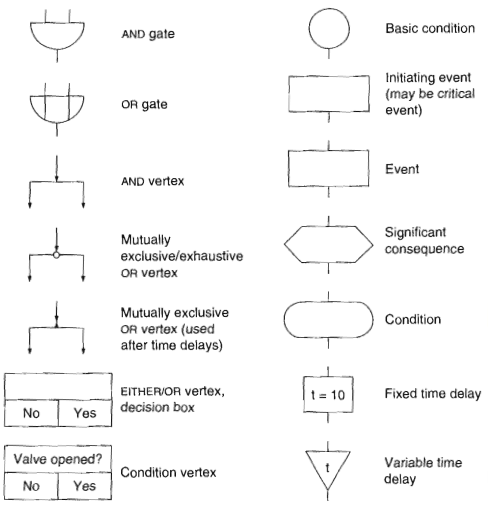
\includegraphics[width=\linewidth]{images/ccaTable.png}
    \end{center}
\end{itemize}

\subsection*{Interface Analysis}
\begin{itemize}
    \item evaluate connections and relationships between components \follows incompatibilities and possibility for common-mode failures
    \item physical, functional or flow category
    \item types of problems
    \begin{itemize}
        \item no output from unit or interconnection failing
        \item degraded output or partial interconnection failure
        \item erratic output (intermittent or unstable operation)
        \item excessive output
        \item unprogrammed output
        \item undesired side effects (e.g. heat damages nearby unit)
    \end{itemize}
    \item similar to HAZOP, but more generalized
\end{itemize}

\subsection*{State Machine Hazard Analysis (SMHA)}
\begin{itemize}
    \item build a state machine, check for hazard state
\end{itemize}

\subsection*{Task and Human Error Analysis}
\subsubsection*{Qualitative Techniques}
\begin{description}
    \item[Procedure Task Analysis] review procedures to verify they are effective and within context for mission task
    \item[Operator Task Analysis] operators task broken down into separate operations
    \item[Action Error Analysis] (AEA) forward search strategy to identify potential deviations in human performance
    \begin{itemize}
        \item potential deviations: forget a step, wrong order of steps, taking too long for a step
    \end{itemize}
    \item[Work Safety Analysis] (WSA) similar to HAZOP, search process is applied to work steps \follows identify hazards and causes
\end{description}

\subsubsection*{Quantitative Techniques}
\begin{itemize}
    \item humand error results from human-task mismatch, poor interfaces, poor operating procedure design
\end{itemize}
\begin{description}
    \item[Simple and Vigilance Tasks] sequence of simple tasks with little to no decision required
    \begin{itemize}
        \item assign probabilities with which the task breaks
        \item series tasks \follows product of probabilities
        \item tree tasks \follows logic combination
        \item also possible: use empirical data for probabilities
    \end{itemize}
    \item[Complex Control Tasks] simple task model inadequate, when technology changes fast \follows decision making, complex problem solving
\end{description}

\end{document}
